\documentclass[dvipdfmx]{jsarticle}
\usepackage[dvipdfmx]{graphicx}
\usepackage{longtable}
\usepackage{lscape}
\usepackage{color}
\usepackage{scalefnt}
%\usepackage{listings,jlisting}
\begin{document}
\title{Abeの\\論文練習}
\author{阿部 衛}
\maketitle{\title}
\thispagestyle{empty}
\newpage 


\section{これが章作成}
章作成はこんな感じ
\subsection{これが節}
この節では、
画像をはる、表を作成することにしてみる

画像貼ります
\begin{figure}[h]
   \begin{center}
     \caption{これが画像だ}
     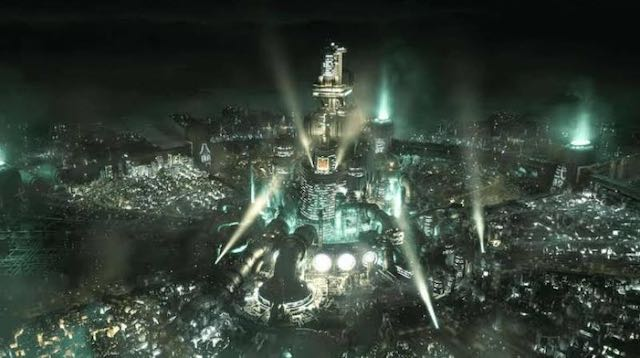
\includegraphics[scale=0.5]{FF7R_zoom.jpg}
 \end{center}
\end{figure}



\begin{table}[h]
 \caption{これが表作成}
 \centering
  \begin{tabular}{|l|r|} \hline
   要素1&要素2\\ \hline \hline
   sample1&sample2\\
   sample3&sample4\\ \hline
\end{tabular}
\end{table}


\newpage 
%参考文献
\begin{thebibliography}{99}
\item
  https://google.com 
\item
 http://www.latex-cmd.com
\end{thebibliography}
\end{document}